% Options for packages loaded elsewhere
\PassOptionsToPackage{unicode}{hyperref}
\PassOptionsToPackage{hyphens}{url}
\PassOptionsToPackage{dvipsnames,svgnames,x11names}{xcolor}
\documentclass[
  10pt,
]{extarticle}
\usepackage{xcolor}
\usepackage[top=1.5in, bottom=1.5in, left=1.5in, right=1.5in]{geometry}
\usepackage{amsmath,amssymb}
\setcounter{secnumdepth}{5}
\usepackage{iftex}
\ifPDFTeX
  \usepackage[T1]{fontenc}
  \usepackage[utf8]{inputenc}
  \usepackage{textcomp} % provide euro and other symbols
\else % if luatex or xetex
  \usepackage{unicode-math} % this also loads fontspec
  \defaultfontfeatures{Scale=MatchLowercase}
  \defaultfontfeatures[\rmfamily]{Ligatures=TeX,Scale=1}
\fi
\usepackage{lmodern}
\ifPDFTeX\else
  % xetex/luatex font selection
\fi
% Use upquote if available, for straight quotes in verbatim environments
\IfFileExists{upquote.sty}{\usepackage{upquote}}{}
\IfFileExists{microtype.sty}{% use microtype if available
  \usepackage[]{microtype}
  \UseMicrotypeSet[protrusion]{basicmath} % disable protrusion for tt fonts
}{}
\makeatletter
\@ifundefined{KOMAClassName}{% if non-KOMA class
  \IfFileExists{parskip.sty}{%
    \usepackage{parskip}
  }{% else
    \setlength{\parindent}{0pt}
    \setlength{\parskip}{6pt plus 2pt minus 1pt}}
}{% if KOMA class
  \KOMAoptions{parskip=half}}
\makeatother
\usepackage{color}
\usepackage{fancyvrb}
\newcommand{\VerbBar}{|}
\newcommand{\VERB}{\Verb[commandchars=\\\{\}]}
\DefineVerbatimEnvironment{Highlighting}{Verbatim}{commandchars=\\\{\}}
% Add ',fontsize=\small' for more characters per line
\usepackage{framed}
\definecolor{shadecolor}{RGB}{248,248,248}
\newenvironment{Shaded}{\begin{snugshade}}{\end{snugshade}}
\newcommand{\AlertTok}[1]{\textcolor[rgb]{0.94,0.16,0.16}{#1}}
\newcommand{\AnnotationTok}[1]{\textcolor[rgb]{0.56,0.35,0.01}{\textbf{\textit{#1}}}}
\newcommand{\AttributeTok}[1]{\textcolor[rgb]{0.13,0.29,0.53}{#1}}
\newcommand{\BaseNTok}[1]{\textcolor[rgb]{0.00,0.00,0.81}{#1}}
\newcommand{\BuiltInTok}[1]{#1}
\newcommand{\CharTok}[1]{\textcolor[rgb]{0.31,0.60,0.02}{#1}}
\newcommand{\CommentTok}[1]{\textcolor[rgb]{0.56,0.35,0.01}{\textit{#1}}}
\newcommand{\CommentVarTok}[1]{\textcolor[rgb]{0.56,0.35,0.01}{\textbf{\textit{#1}}}}
\newcommand{\ConstantTok}[1]{\textcolor[rgb]{0.56,0.35,0.01}{#1}}
\newcommand{\ControlFlowTok}[1]{\textcolor[rgb]{0.13,0.29,0.53}{\textbf{#1}}}
\newcommand{\DataTypeTok}[1]{\textcolor[rgb]{0.13,0.29,0.53}{#1}}
\newcommand{\DecValTok}[1]{\textcolor[rgb]{0.00,0.00,0.81}{#1}}
\newcommand{\DocumentationTok}[1]{\textcolor[rgb]{0.56,0.35,0.01}{\textbf{\textit{#1}}}}
\newcommand{\ErrorTok}[1]{\textcolor[rgb]{0.64,0.00,0.00}{\textbf{#1}}}
\newcommand{\ExtensionTok}[1]{#1}
\newcommand{\FloatTok}[1]{\textcolor[rgb]{0.00,0.00,0.81}{#1}}
\newcommand{\FunctionTok}[1]{\textcolor[rgb]{0.13,0.29,0.53}{\textbf{#1}}}
\newcommand{\ImportTok}[1]{#1}
\newcommand{\InformationTok}[1]{\textcolor[rgb]{0.56,0.35,0.01}{\textbf{\textit{#1}}}}
\newcommand{\KeywordTok}[1]{\textcolor[rgb]{0.13,0.29,0.53}{\textbf{#1}}}
\newcommand{\NormalTok}[1]{#1}
\newcommand{\OperatorTok}[1]{\textcolor[rgb]{0.81,0.36,0.00}{\textbf{#1}}}
\newcommand{\OtherTok}[1]{\textcolor[rgb]{0.56,0.35,0.01}{#1}}
\newcommand{\PreprocessorTok}[1]{\textcolor[rgb]{0.56,0.35,0.01}{\textit{#1}}}
\newcommand{\RegionMarkerTok}[1]{#1}
\newcommand{\SpecialCharTok}[1]{\textcolor[rgb]{0.81,0.36,0.00}{\textbf{#1}}}
\newcommand{\SpecialStringTok}[1]{\textcolor[rgb]{0.31,0.60,0.02}{#1}}
\newcommand{\StringTok}[1]{\textcolor[rgb]{0.31,0.60,0.02}{#1}}
\newcommand{\VariableTok}[1]{\textcolor[rgb]{0.00,0.00,0.00}{#1}}
\newcommand{\VerbatimStringTok}[1]{\textcolor[rgb]{0.31,0.60,0.02}{#1}}
\newcommand{\WarningTok}[1]{\textcolor[rgb]{0.56,0.35,0.01}{\textbf{\textit{#1}}}}
\usepackage{longtable,booktabs,array}
\usepackage{calc} % for calculating minipage widths
% Correct order of tables after \paragraph or \subparagraph
\usepackage{etoolbox}
\makeatletter
\patchcmd\longtable{\par}{\if@noskipsec\mbox{}\fi\par}{}{}
\makeatother
% Allow footnotes in longtable head/foot
\IfFileExists{footnotehyper.sty}{\usepackage{footnotehyper}}{\usepackage{footnote}}
\makesavenoteenv{longtable}
\usepackage{graphicx}
\makeatletter
\newsavebox\pandoc@box
\newcommand*\pandocbounded[1]{% scales image to fit in text height/width
  \sbox\pandoc@box{#1}%
  \Gscale@div\@tempa{\textheight}{\dimexpr\ht\pandoc@box+\dp\pandoc@box\relax}%
  \Gscale@div\@tempb{\linewidth}{\wd\pandoc@box}%
  \ifdim\@tempb\p@<\@tempa\p@\let\@tempa\@tempb\fi% select the smaller of both
  \ifdim\@tempa\p@<\p@\scalebox{\@tempa}{\usebox\pandoc@box}%
  \else\usebox{\pandoc@box}%
  \fi%
}
% Set default figure placement to htbp
\def\fps@figure{htbp}
\makeatother
\setlength{\emergencystretch}{3em} % prevent overfull lines
\providecommand{\tightlist}{%
  \setlength{\itemsep}{0pt}\setlength{\parskip}{0pt}}
\usepackage{xcolor}
\usepackage{hyperref}
\hypersetup{colorlinks=true, linkcolor=blue, urlcolor=blue, citecolor=blue}
\usepackage{float}
\usepackage{fvextra}
\usepackage{xcolor}
\usepackage{fancyhdr}
\usepackage{lastpage}
\usepackage{soul}
\usepackage{etoolbox}
\usepackage{microtype}
\usepackage{tcolorbox}
\usepackage{enumitem}
\usepackage{fancyvrb}
\usepackage{xspace}
\allowdisplaybreaks
\setcounter{tocdepth}{2}
\setcounter{secnumdepth}{0}
\floatplacement{figure}{H}
\makeatletter
\newcommand{\@subtitle}{}
\newcommand{\subtitle}[1]{\gdef\@subtitle{#1}}
\newcommand{\DocSubtitle}{\@subtitle}
\renewcommand{\maketitle}{
  \thispagestyle{plain}
  \null
  \vfill
  \begin{center}
    {\Large \textsc{\@title} \par}\vskip 0.5em
    {\LARGE \bfseries \@subtitle \par}\vskip 0.75em
    {\large \@author \par}\vskip 0.5em
    {\normalsize \@date \par}
  \end{center}
  \vfill
  \tableofcontents
  \vspace{1em}
  \clearpage
}
\AfterEndEnvironment{Highlighting}{\setcounter{CodeLine}{\numexpr\value{CodeLine}+\FV@CodeLineNo\relax}}
\makeatother
\fancypagestyle{plain}{
  \fancyhf{}
  \renewcommand{\headrulewidth}{0pt}
  \renewcommand{\footrulewidth}{0pt}
}
\pagestyle{fancy}
\fancyhf{}
\fancyfoot[C]{\small\textsc{Page}~\thepage~\textsc{of}~\pageref{LastPage}}
\fancyhead[L]{\textsc{Rento Saijo}}
\fancyhead[R]{\textsc{\DocSubtitle}}
\fancyhead[C]{\textsc{\rightmark}}
\renewcommand{\headrulewidth}{0.5pt}
\renewcommand{\footrulewidth}{0.5pt}
\newcounter{CodeLine}
\newcounter{cell}
\AtBeginEnvironment{Highlighting}{\stepcounter{cell}}
\DefineVerbatimEnvironment{Highlighting}{Verbatim}{
  frame=single,
  rulecolor=\color{black},
  framesep=2mm,
  label=\footnotesize\textbf{Cell \thecell},
  labelposition=topline,
  commandchars=\\\{\},
  breaklines=true,
  breakanywhere=false,
  breaksymbol={},
  numbers=left,
  numbersep=3pt,
  firstnumber=\numexpr\value{CodeLine}+1\relax,
  fontsize=\small
}
\DefineVerbatimEnvironment{verbatim}{Verbatim}{
  breaklines=true,
  breakanywhere=true,
  numbers=left,
  numbersep=3pt,
  firstnumber=1,
  fontsize=\footnotesize
}
\DefineVerbatimEnvironment{snippet}{Verbatim}{
  breaklines=true,
  breakanywhere=true,
  fontsize=\footnotesize,
  frame=single,
  listparameters=\setlength{\topsep}{\baselineskip}\setlength{\partopsep}{0pt}
}
\newtcolorbox{problem}[1][]{
  title={\textsc{#1}}
}
\newenvironment{alphenum}{
  \begin{enumerate}[
    label=(\alph*),
    itemsep=3pt,
    parsep=0pt,
    topsep=6pt
  ]
}{
  \end{enumerate}
}
\newenvironment{items}{
  \begin{itemize}[
    itemsep=3pt,
    parsep=0pt,
    topsep=6pt
  ]
}{
  \end{itemize}
}
\renewcommand{\contentsname}{Table of Contents}
\newcommand{\E}{\mathrm{E}}
\newcommand{\Var}{\mathrm{Var}}
\newcommand{\R}{\textsf{R}\xspace}
\newcommand{\Pois}{\mathrm{Pois}}
\newcommand{\SD}{\mathrm{SD}}
\newcommand{\SE}{\mathrm{SE}}
\usepackage{bookmark}
\IfFileExists{xurl.sty}{\usepackage{xurl}}{} % add URL line breaks if available
\urlstyle{same}
\hypersetup{
  pdftitle={STA 209: Introduction to Time Series Analysis},
  colorlinks=true,
  linkcolor={blue},
  filecolor={Maroon},
  citecolor={blue},
  urlcolor={blue},
  pdfcreator={LaTeX via pandoc}}

\title{STA 209: Introduction to Time Series Analysis}
\usepackage{etoolbox}
\makeatletter
\providecommand{\subtitle}[1]{% add subtitle to \maketitle
  \apptocmd{\@title}{\par {\large #1 \par}}{}{}
}
\makeatother
\subtitle{Homework 2}
\author{Rento Saijo}
\date{February 19, 2026}

\begin{document}
\maketitle

\section{Disclosure}\label{disclosure}

GPT-5.3-Codex was used to create the \texttt{YAML} portion and some \texttt{LaTeX} code to format the text/equations nicely. Page formatting code was also provided by Derin Gezgin. In the setup chunk, libraries were loaded and some helper functions were defined including but not limited to \texttt{table\_latex()} and \texttt{with\_family()}. See the original \texttt{RMD} file \href{https://github.com/RentoSaijo/STA209/blob/main/Homework2.Rmd}{here} for more details.

\newpage

\section{Problem 1}\label{problem-1}

\begin{problem}[Problem 1]
Consider the Southern oscillation index data (\texttt{soi}) from Homework 1. Use this data to do the following in R and report your results. Use periodicity \(s = 12\). Fit the following five models:
\begin{align*}
\textbf{Model I:}\quad
\text{SOI}_t
&= \beta_0 + \beta_1 t + W_t,\\
\textbf{Model II:}\quad
\text{SOI}_t
&= \beta_0 + \beta_1 t + \frac{\beta_2 t^2}{2!} + W_t,\\
\textbf{Model III:}\quad
\text{SOI}_t
&= \beta_0 + \alpha_1\cos\!\left(\frac{2\pi t}{s}\right) + \alpha_2\sin\!\left(\frac{2\pi t}{s}\right) + W_t,\\
\textbf{Model IV:}\quad
\text{SOI}_t
&= \beta_0 + \beta_1 t + \alpha_1\cos\!\left(\frac{2\pi t}{s}\right) + \alpha_2\sin\!\left(\frac{2\pi t}{s}\right) + W_t,\\
\textbf{Model V:}\quad
\text{SOI}_t
&= \beta_0 + \beta_1 t
+ \alpha_1\cos\!\left(\frac{2\pi t}{s}\right)
+ \alpha_2\sin\!\left(\frac{2\pi t}{s}\right)\\
&\quad + \alpha_3\cos\!\left(\frac{4\pi t}{s}\right)
+ \alpha_4\sin\!\left(\frac{4\pi t}{s}\right)
+ W_t.
\end{align*}
\end{problem}

The Southern Oscillation Index (SOI) dataset is a monthly time series with 453 observations covering the years 1950 through 1987. It is represented in the form \texttt{Time-Series [1:453]} (notated as running from 1950 to 1988 in the printed format) and is shown as a numeric sequence (e.g., \texttt{0.377, 0.246, 0.311, 0.104, -0.016, 0.235, \dots}). The series is intended to pair with \texttt{rec} (Recruitment) for related analyses. The data were furnished by Dr.~Roy Mendelssohn of the Pacific Fisheries Environmental Laboratory, NOAA (personal communication). Demonstrations of \texttt{astsa} capabilities are referenced under \emph{FUN WITH ASTSA}, and the most recent version of the package is maintained on GitHub along with the \texttt{NEWS} and \texttt{ChangeLog} files; additional webpages for the associated texts and help using \textsf{R} for time series analysis are available at the author's site.

\newpage

\subsection{Problem 1 (a)}\label{problem-1-a}

\begin{problem}[Problem 1 (a)]
Report the five fitted models.
\end{problem}

\begin{Shaded}
\begin{Highlighting}[]
\CommentTok{\# Load SOI data and define periodicity.}
\FunctionTok{data}\NormalTok{(soi)}
\NormalTok{s }\OtherTok{\textless{}{-}} \DecValTok{12}
\NormalTok{Y }\OtherTok{\textless{}{-}}\NormalTok{ soi}
\NormalTok{t }\OtherTok{\textless{}{-}} \FunctionTok{time}\NormalTok{(Y)}
\NormalTok{ts2 }\OtherTok{\textless{}{-}}\NormalTok{ t}\SpecialCharTok{\^{}}\DecValTok{2} \SpecialCharTok{/} \FunctionTok{factorial}\NormalTok{(}\DecValTok{2}\NormalTok{)}
\NormalTok{cs1 }\OtherTok{\textless{}{-}} \FunctionTok{cos}\NormalTok{(}\DecValTok{2} \SpecialCharTok{*}\NormalTok{ pi }\SpecialCharTok{*}\NormalTok{ t }\SpecialCharTok{/}\NormalTok{ s)}
\NormalTok{sn1 }\OtherTok{\textless{}{-}} \FunctionTok{sin}\NormalTok{(}\DecValTok{2} \SpecialCharTok{*}\NormalTok{ pi }\SpecialCharTok{*}\NormalTok{ t }\SpecialCharTok{/}\NormalTok{ s)}
\NormalTok{cs2 }\OtherTok{\textless{}{-}} \FunctionTok{cos}\NormalTok{(}\DecValTok{4} \SpecialCharTok{*}\NormalTok{ pi }\SpecialCharTok{*}\NormalTok{ t }\SpecialCharTok{/}\NormalTok{ s)}
\NormalTok{sn2 }\OtherTok{\textless{}{-}} \FunctionTok{sin}\NormalTok{(}\DecValTok{4} \SpecialCharTok{*}\NormalTok{ pi }\SpecialCharTok{*}\NormalTok{ t }\SpecialCharTok{/}\NormalTok{ s)}

\CommentTok{\# Fit all five models.}
\NormalTok{m1 }\OtherTok{\textless{}{-}} \FunctionTok{lm}\NormalTok{(Y }\SpecialCharTok{\textasciitilde{}}\NormalTok{ t)}
\NormalTok{m2 }\OtherTok{\textless{}{-}} \FunctionTok{lm}\NormalTok{(Y }\SpecialCharTok{\textasciitilde{}}\NormalTok{ t }\SpecialCharTok{+}\NormalTok{ ts2)}
\NormalTok{m3 }\OtherTok{\textless{}{-}} \FunctionTok{lm}\NormalTok{(Y }\SpecialCharTok{\textasciitilde{}}\NormalTok{ cs1 }\SpecialCharTok{+}\NormalTok{ sn1)}
\NormalTok{m4 }\OtherTok{\textless{}{-}} \FunctionTok{lm}\NormalTok{(Y }\SpecialCharTok{\textasciitilde{}}\NormalTok{ t }\SpecialCharTok{+}\NormalTok{ cs1 }\SpecialCharTok{+}\NormalTok{ sn1)}
\NormalTok{m5 }\OtherTok{\textless{}{-}} \FunctionTok{lm}\NormalTok{(Y }\SpecialCharTok{\textasciitilde{}}\NormalTok{ t }\SpecialCharTok{+}\NormalTok{ cs1 }\SpecialCharTok{+}\NormalTok{ sn1 }\SpecialCharTok{+}\NormalTok{ cs2 }\SpecialCharTok{+}\NormalTok{ sn2)}

\CommentTok{\# See model summaries.}
\FunctionTok{summary}\NormalTok{(m1)}
\end{Highlighting}
\end{Shaded}

\begin{verbatim}
## 
## Call:
## lm(formula = Y ~ t)
## 
## Residuals:
##      Min       1Q   Median       3Q      Max 
## -1.04140 -0.24183  0.01935  0.27727  0.83866 
## 
## Coefficients:
##             Estimate Std. Error t value  Pr(>|t|)    
## (Intercept) 13.70367    3.18873   4.298 0.0000212 ***
## t           -0.00692    0.00162  -4.272 0.0000236 ***
## ---
## Signif. codes:  0 '***' 0.001 '**' 0.01 '*' 0.05 '.' 0.1 ' ' 1
## 
## Residual standard error: 0.3756 on 451 degrees of freedom
## Multiple R-squared:  0.0389, Adjusted R-squared:  0.03677 
## F-statistic: 18.25 on 1 and 451 DF,  p-value: 0.00002359
\end{verbatim}

\begin{Shaded}
\begin{Highlighting}[]
\FunctionTok{summary}\NormalTok{(m2)}
\end{Highlighting}
\end{Shaded}

\begin{verbatim}
## 
## Call:
## lm(formula = Y ~ t + ts2)
## 
## Residuals:
##     Min      1Q  Median      3Q     Max 
## -1.0529 -0.2443  0.0129  0.2658  0.8412 
## 
## Coefficients:
##                 Estimate   Std. Error t value Pr(>|t|)
## (Intercept) -496.7608959  644.3532809  -0.771    0.441
## t              0.5116415    0.6545674   0.782    0.435
## ts2           -0.0002634    0.0003325  -0.792    0.429
## 
## Residual standard error: 0.3758 on 450 degrees of freedom
## Multiple R-squared:  0.04024,    Adjusted R-squared:  0.03597 
## F-statistic: 9.433 on 2 and 450 DF,  p-value: 0.00009698
\end{verbatim}

\begin{Shaded}
\begin{Highlighting}[]
\FunctionTok{summary}\NormalTok{(m3)}
\end{Highlighting}
\end{Shaded}

\begin{verbatim}
## 
## Call:
## lm(formula = Y ~ cs1 + sn1)
## 
## Residuals:
##      Min       1Q   Median       3Q      Max 
## -1.08705 -0.26231  0.03387  0.28045  0.93815 
## 
## Coefficients:
##               Estimate Std. Error t value  Pr(>|t|)    
## (Intercept)  0.0794096  0.0180282   4.405 0.0000133 ***
## cs1         -0.0008964  0.0251756  -0.036     0.972    
## sn1         -0.0312776  0.0258020  -1.212     0.226    
## ---
## Signif. codes:  0 '***' 0.001 '**' 0.01 '*' 0.05 '.' 0.1 ' ' 1
## 
## Residual standard error: 0.383 on 450 degrees of freedom
## Multiple R-squared:  0.003266,   Adjusted R-squared:  -0.001164 
## F-statistic: 0.7373 on 2 and 450 DF,  p-value: 0.479
\end{verbatim}

\begin{Shaded}
\begin{Highlighting}[]
\FunctionTok{summary}\NormalTok{(m4)}
\end{Highlighting}
\end{Shaded}

\begin{verbatim}
## 
## Call:
## lm(formula = Y ~ t + cs1 + sn1)
## 
## Residuals:
##     Min      1Q  Median      3Q     Max 
## -1.0538 -0.2431  0.0269  0.2770  0.8546 
## 
## Coefficients:
##              Estimate Std. Error t value  Pr(>|t|)    
## (Intercept) 13.575646   3.271475   4.150 0.0000398 ***
## t           -0.006855   0.001662  -4.125 0.0000441 ***
## cs1         -0.010721   0.024854  -0.431     0.666    
## sn1         -0.010208   0.025864  -0.395     0.693    
## ---
## Signif. codes:  0 '***' 0.001 '**' 0.01 '*' 0.05 '.' 0.1 ' ' 1
## 
## Residual standard error: 0.3763 on 449 degrees of freedom
## Multiple R-squared:  0.03967,    Adjusted R-squared:  0.03325 
## F-statistic: 6.182 on 3 and 449 DF,  p-value: 0.0004011
\end{verbatim}

\begin{Shaded}
\begin{Highlighting}[]
\FunctionTok{summary}\NormalTok{(m5)}
\end{Highlighting}
\end{Shaded}

\begin{verbatim}
## 
## Call:
## lm(formula = Y ~ t + cs1 + sn1 + cs2 + sn2)
## 
## Residuals:
##      Min       1Q   Median       3Q      Max 
## -1.06440 -0.24486  0.01442  0.27100  0.84117 
## 
## Coefficients:
##              Estimate Std. Error t value  Pr(>|t|)    
## (Intercept) 12.797341   3.238141   3.952 0.0000900 ***
## t           -0.006460   0.001645  -3.928 0.0000992 ***
## cs1         -0.008360   0.024591  -0.340    0.7340    
## sn1         -0.009441   0.025548  -0.370    0.7119    
## cs2         -0.043304   0.024829  -1.744    0.0818 .  
## sn2          0.081218   0.024730   3.284    0.0011 ** 
## ---
## Signif. codes:  0 '***' 0.001 '**' 0.01 '*' 0.05 '.' 0.1 ' ' 1
## 
## Residual standard error: 0.3716 on 447 degrees of freedom
## Multiple R-squared:  0.06798,    Adjusted R-squared:  0.05755 
## F-statistic:  6.52 on 5 and 447 DF,  p-value: 0.000007219
\end{verbatim}

The fitted models are:
\begin{align*}
\widehat{\textbf{Model I:}}\quad
\widehat{\text{SOI}}_t
&= 13.704 - 0.007\,t,\\[4pt]
\widehat{\textbf{Model II:}}\quad
\widehat{\text{SOI}}_t
&= -496.761 + 0.512\,t - 0.000\,\frac{t^2}{2!},\\[4pt]
\widehat{\textbf{Model III:}}\quad
\widehat{\text{SOI}}_t
&= 0.079 - 0.001\,\cos\!\left(\frac{2\pi t}{12}\right) - 0.031\,\sin\!\left(\frac{2\pi t}{12}\right),\\[4pt]
\widehat{\textbf{Model IV:}}\quad
\widehat{\text{SOI}}_t
&= 13.576 - 0.007\,t - 0.011\,\cos\!\left(\frac{2\pi t}{12}\right) - 0.010\,\sin\!\left(\frac{2\pi t}{12}\right),\\[4pt]
\widehat{\textbf{Model V:}}\quad
\widehat{\text{SOI}}_t
&= 12.797 - 0.006\,t - 0.008\,\cos\!\left(\frac{2\pi t}{12}\right) - 0.009\,\sin\!\left(\frac{2\pi t}{12}\right)\\
&\quad - 0.043\,\cos\!\left(\frac{4\pi t}{12}\right) + 0.081\,\sin\!\left(\frac{4\pi t}{12}\right),
\end{align*}
where \(\text{SOI}_t\) denotes the Southern Oscillation Index at time \(t\).

\newpage

\subsection{Problem 1 (b)}\label{problem-1-b}

\begin{problem}[Problem 1 (b)]
Prepare a summary table using number of regression parameters, \(R_a^2\), AIC, AICC and BIC.
\end{problem}

\begin{Shaded}
\begin{Highlighting}[]
\CommentTok{\# Build table of fit criteria.}
\NormalTok{fit\_table }\OtherTok{\textless{}{-}} \ControlFlowTok{function}\NormalTok{(fit) \{}
\NormalTok{  n   }\OtherTok{\textless{}{-}} \FunctionTok{length}\NormalTok{(}\FunctionTok{resid}\NormalTok{(fit))}
\NormalTok{  r   }\OtherTok{\textless{}{-}} \FunctionTok{length}\NormalTok{(}\FunctionTok{coef}\NormalTok{(fit))}
\NormalTok{  sse }\OtherTok{\textless{}{-}} \FunctionTok{sum}\NormalTok{(}\FunctionTok{resid}\NormalTok{(fit)}\SpecialCharTok{\^{}}\DecValTok{2}\NormalTok{)}
  \FunctionTok{data.frame}\NormalTok{(}
    \AttributeTok{Parameters =}\NormalTok{ r,}
    \AttributeTok{R2a  =} \FunctionTok{summary}\NormalTok{(fit)}\SpecialCharTok{$}\NormalTok{adj.r.squared,}
    \AttributeTok{AIC  =} \FunctionTok{AIC}\NormalTok{(fit) }\SpecialCharTok{/}\NormalTok{ n,}
    \AttributeTok{AICC =} \FunctionTok{log}\NormalTok{(sse }\SpecialCharTok{/}\NormalTok{ n) }\SpecialCharTok{+}\NormalTok{ ((n }\SpecialCharTok{+}\NormalTok{ r) }\SpecialCharTok{/}\NormalTok{ (n }\SpecialCharTok{{-}}\NormalTok{ r }\SpecialCharTok{{-}} \DecValTok{2}\NormalTok{)),}
    \AttributeTok{BIC  =} \FunctionTok{AIC}\NormalTok{(fit, }\AttributeTok{k =} \FunctionTok{log}\NormalTok{(n)) }\SpecialCharTok{/}\NormalTok{ n}
\NormalTok{  )}
\NormalTok{\}}
\NormalTok{comp1 }\OtherTok{\textless{}{-}}\NormalTok{ dplyr}\SpecialCharTok{::}\FunctionTok{bind\_rows}\NormalTok{(}
  \StringTok{\textquotesingle{}Model I\textquotesingle{}}   \OtherTok{=} \FunctionTok{fit\_table}\NormalTok{(m1),}
  \StringTok{\textquotesingle{}Model II\textquotesingle{}}  \OtherTok{=} \FunctionTok{fit\_table}\NormalTok{(m2),}
  \StringTok{\textquotesingle{}Model III\textquotesingle{}} \OtherTok{=} \FunctionTok{fit\_table}\NormalTok{(m3),}
  \StringTok{\textquotesingle{}Model IV\textquotesingle{}}  \OtherTok{=} \FunctionTok{fit\_table}\NormalTok{(m4),}
  \StringTok{\textquotesingle{}Model V\textquotesingle{}}   \OtherTok{=} \FunctionTok{fit\_table}\NormalTok{(m5),}
  \AttributeTok{.id =} \StringTok{\textquotesingle{}Model\textquotesingle{}}
\NormalTok{)}
\NormalTok{comp1}\SpecialCharTok{$}\NormalTok{Parameters }\OtherTok{\textless{}{-}} \FunctionTok{as.integer}\NormalTok{(comp1}\SpecialCharTok{$}\NormalTok{Parameters)}
\NormalTok{comp1 }\OtherTok{\textless{}{-}}\NormalTok{ comp1 }\SpecialCharTok{\%\textgreater{}\%}
\NormalTok{  dplyr}\SpecialCharTok{::}\FunctionTok{mutate}\NormalTok{(}
    \AttributeTok{R2a  =} \FunctionTok{round}\NormalTok{(R2a, }\DecValTok{3}\NormalTok{),}
    \AttributeTok{AIC  =} \FunctionTok{round}\NormalTok{(AIC, }\DecValTok{3}\NormalTok{),}
    \AttributeTok{AICC =} \FunctionTok{round}\NormalTok{(AICC, }\DecValTok{3}\NormalTok{),}
    \AttributeTok{BIC  =} \FunctionTok{round}\NormalTok{(BIC, }\DecValTok{3}\NormalTok{)}
\NormalTok{  )}
\FunctionTok{table\_latex}\NormalTok{(comp1, }\AttributeTok{col\_names =} \FunctionTok{c}\NormalTok{(}\StringTok{\textquotesingle{}Model\textquotesingle{}}\NormalTok{, }\StringTok{\textquotesingle{}}\SpecialCharTok{\textbackslash{}\textbackslash{}}\StringTok{\# Parameters\textquotesingle{}}\NormalTok{, }\StringTok{\textquotesingle{}$R\_a\^{}2$\textquotesingle{}}\NormalTok{, }\StringTok{\textquotesingle{}AIC\textquotesingle{}}\NormalTok{, }\StringTok{\textquotesingle{}AICC\textquotesingle{}}\NormalTok{, }\StringTok{\textquotesingle{}BIC\textquotesingle{}}\NormalTok{))}
\end{Highlighting}
\end{Shaded}

\begin{table}[H]
\centering
\begin{tabular}{cccccc}
\toprule
Model & \# Parameters & $R_a^2$ & AIC & AICC & BIC\\
\midrule
Model I & 2 & 0.037 & 0.888 & -0.949 & 0.916\\
Model II & 3 & 0.036 & 0.891 & -0.946 & 0.928\\
Model III & 3 & -0.001 & 0.929 & -0.908 & 0.966\\
Model IV & 4 & 0.033 & 0.897 & -0.941 & 0.942\\
Model V & 6 & 0.058 & 0.875 & -0.962 & 0.939\\
\bottomrule
\end{tabular}
\end{table}

\newpage

\subsection{Problem 1 (c)}\label{problem-1-c}

\begin{problem}[Problem 1 (c)]
Using the summary in (b), which model is selected to explain SOI and why?
\end{problem}

For explanation, we prioritize adjusted \(R^2\). Model V has the largest adjusted \(R^2\), with \(R_a^2 = 0.058\). Also, its overall F-test is significant with \(F = 6.520\) and \(p = 0.000\) (although all others have fairly low values as well). All in all, though, \textbf{Model V} is selected for explaining SOI variation among these candidates.

\newpage

\subsection{Problem 1 (d)}\label{problem-1-d}

\begin{problem}[Problem 1 (d)]
Based on AIC, AICC and BIC, which model is selected and what is it best for?
\end{problem}

AIC and AICC are minimized by \textbf{Model V}, with \(AIC = 0.875\) and \(AICC = -0.962\), but BIC is minimized by \textbf{Model I}, with \(BIC = 0.916\). Since these criteria disagree and BIC applies the strongest complexity penalty, we select \textbf{Model I}. This selected model maximizes the probability that the sample data are from the suggested model.

\newpage

\subsection{Problem 1 (e)}\label{problem-1-e}

\begin{problem}[Problem 1 (e)]
Remove the last 30 values and compare future forecast error across models using ME, MPE, MSE, MAE, and MAPE. Include these with \(R_a^2\), AIC, AICC and BIC in a table. Does the selected model match part (c)?
\end{problem}

\begin{Shaded}
\begin{Highlighting}[]
\CommentTok{\# Hold out the last 30 observations.}
\NormalTok{h     }\OtherTok{\textless{}{-}} \DecValTok{30}
\NormalTok{n\_all }\OtherTok{\textless{}{-}} \FunctionTok{length}\NormalTok{(Y)}
\NormalTok{cut   }\OtherTok{\textless{}{-}}\NormalTok{ n\_all }\SpecialCharTok{{-}}\NormalTok{ h}
\NormalTok{Y\_train   }\OtherTok{\textless{}{-}}\NormalTok{ stats}\SpecialCharTok{::}\FunctionTok{window}\NormalTok{(Y, }\AttributeTok{end =} \FunctionTok{time}\NormalTok{(Y)[cut])}
\NormalTok{Y\_test    }\OtherTok{\textless{}{-}}\NormalTok{ stats}\SpecialCharTok{::}\FunctionTok{window}\NormalTok{(Y, }\AttributeTok{start =} \FunctionTok{time}\NormalTok{(Y)[cut }\SpecialCharTok{+} \DecValTok{1}\NormalTok{])}
\NormalTok{t\_train   }\OtherTok{\textless{}{-}} \FunctionTok{time}\NormalTok{(Y\_train)}
\NormalTok{t\_test    }\OtherTok{\textless{}{-}} \FunctionTok{time}\NormalTok{(Y\_test)}
\NormalTok{ts2\_train }\OtherTok{\textless{}{-}}\NormalTok{ t\_train}\SpecialCharTok{\^{}}\DecValTok{2} \SpecialCharTok{/} \FunctionTok{factorial}\NormalTok{(}\DecValTok{2}\NormalTok{)}
\NormalTok{ts2\_test  }\OtherTok{\textless{}{-}}\NormalTok{ t\_test}\SpecialCharTok{\^{}}\DecValTok{2} \SpecialCharTok{/} \FunctionTok{factorial}\NormalTok{(}\DecValTok{2}\NormalTok{)}
\NormalTok{cs1\_train }\OtherTok{\textless{}{-}} \FunctionTok{cos}\NormalTok{(}\DecValTok{2} \SpecialCharTok{*}\NormalTok{ pi }\SpecialCharTok{*}\NormalTok{ t\_train }\SpecialCharTok{/}\NormalTok{ s)}
\NormalTok{sn1\_train }\OtherTok{\textless{}{-}} \FunctionTok{sin}\NormalTok{(}\DecValTok{2} \SpecialCharTok{*}\NormalTok{ pi }\SpecialCharTok{*}\NormalTok{ t\_train }\SpecialCharTok{/}\NormalTok{ s)}
\NormalTok{cs2\_train }\OtherTok{\textless{}{-}} \FunctionTok{cos}\NormalTok{(}\DecValTok{4} \SpecialCharTok{*}\NormalTok{ pi }\SpecialCharTok{*}\NormalTok{ t\_train }\SpecialCharTok{/}\NormalTok{ s)}
\NormalTok{sn2\_train }\OtherTok{\textless{}{-}} \FunctionTok{sin}\NormalTok{(}\DecValTok{4} \SpecialCharTok{*}\NormalTok{ pi }\SpecialCharTok{*}\NormalTok{ t\_train }\SpecialCharTok{/}\NormalTok{ s)}
\NormalTok{cs1\_test  }\OtherTok{\textless{}{-}} \FunctionTok{cos}\NormalTok{(}\DecValTok{2} \SpecialCharTok{*}\NormalTok{ pi }\SpecialCharTok{*}\NormalTok{ t\_test }\SpecialCharTok{/}\NormalTok{ s)}
\NormalTok{sn1\_test  }\OtherTok{\textless{}{-}} \FunctionTok{sin}\NormalTok{(}\DecValTok{2} \SpecialCharTok{*}\NormalTok{ pi }\SpecialCharTok{*}\NormalTok{ t\_test }\SpecialCharTok{/}\NormalTok{ s)}
\NormalTok{cs2\_test  }\OtherTok{\textless{}{-}} \FunctionTok{cos}\NormalTok{(}\DecValTok{4} \SpecialCharTok{*}\NormalTok{ pi }\SpecialCharTok{*}\NormalTok{ t\_test }\SpecialCharTok{/}\NormalTok{ s)}
\NormalTok{sn2\_test  }\OtherTok{\textless{}{-}} \FunctionTok{sin}\NormalTok{(}\DecValTok{4} \SpecialCharTok{*}\NormalTok{ pi }\SpecialCharTok{*}\NormalTok{ t\_test }\SpecialCharTok{/}\NormalTok{ s)}

\CommentTok{\# Refit on training data.}
\NormalTok{f1 }\OtherTok{\textless{}{-}} \FunctionTok{lm}\NormalTok{(Y\_train }\SpecialCharTok{\textasciitilde{}}\NormalTok{ t\_train)}
\NormalTok{f2 }\OtherTok{\textless{}{-}} \FunctionTok{lm}\NormalTok{(Y\_train }\SpecialCharTok{\textasciitilde{}}\NormalTok{ t\_train }\SpecialCharTok{+}\NormalTok{ ts2\_train)}
\NormalTok{f3 }\OtherTok{\textless{}{-}} \FunctionTok{lm}\NormalTok{(Y\_train }\SpecialCharTok{\textasciitilde{}}\NormalTok{ cs1\_train }\SpecialCharTok{+}\NormalTok{ sn1\_train)}
\NormalTok{f4 }\OtherTok{\textless{}{-}} \FunctionTok{lm}\NormalTok{(Y\_train }\SpecialCharTok{\textasciitilde{}}\NormalTok{ t\_train }\SpecialCharTok{+}\NormalTok{ cs1\_train }\SpecialCharTok{+}\NormalTok{ sn1\_train)}
\NormalTok{f5 }\OtherTok{\textless{}{-}} \FunctionTok{lm}\NormalTok{(Y\_train }\SpecialCharTok{\textasciitilde{}}\NormalTok{ t\_train }\SpecialCharTok{+}\NormalTok{ cs1\_train }\SpecialCharTok{+}\NormalTok{ sn1\_train }\SpecialCharTok{+}\NormalTok{ cs2\_train }\SpecialCharTok{+}\NormalTok{ sn2\_train)}

\CommentTok{\# Forecast the held{-}out 30 observations.}
\NormalTok{p1 }\OtherTok{\textless{}{-}} \FunctionTok{predict}\NormalTok{(f1, }\AttributeTok{newdata =} \FunctionTok{data.frame}\NormalTok{(}\AttributeTok{t\_train =}\NormalTok{ t\_test))}
\NormalTok{p2 }\OtherTok{\textless{}{-}} \FunctionTok{predict}\NormalTok{(f2, }\AttributeTok{newdata =} \FunctionTok{data.frame}\NormalTok{(}\AttributeTok{t\_train =}\NormalTok{ t\_test, }\AttributeTok{ts2\_train =}\NormalTok{ ts2\_test))}
\NormalTok{p3 }\OtherTok{\textless{}{-}} \FunctionTok{predict}\NormalTok{(f3, }\AttributeTok{newdata =} \FunctionTok{data.frame}\NormalTok{(}\AttributeTok{cs1\_train =}\NormalTok{ cs1\_test, }\AttributeTok{sn1\_train =}\NormalTok{ sn1\_test))}
\NormalTok{p4 }\OtherTok{\textless{}{-}} \FunctionTok{predict}\NormalTok{(f4, }\AttributeTok{newdata =} \FunctionTok{data.frame}\NormalTok{(}\AttributeTok{t\_train =}\NormalTok{ t\_test, }\AttributeTok{cs1\_train =}\NormalTok{ cs1\_test, }\AttributeTok{sn1\_train =}\NormalTok{ sn1\_test))}
\NormalTok{p5 }\OtherTok{\textless{}{-}} \FunctionTok{predict}\NormalTok{(f5, }\AttributeTok{newdata =} \FunctionTok{data.frame}\NormalTok{(}\AttributeTok{t\_train =}\NormalTok{ t\_test, }\AttributeTok{cs1\_train =}\NormalTok{ cs1\_test, }\AttributeTok{sn1\_train =}\NormalTok{ sn1\_test, }\AttributeTok{cs2\_train =}\NormalTok{ cs2\_test, }\AttributeTok{sn2\_train =}\NormalTok{ sn2\_test))}

\CommentTok{\# Forecast error metrics (Lecture 5 style).}
\NormalTok{fcst\_metrics }\OtherTok{\textless{}{-}} \ControlFlowTok{function}\NormalTok{(y\_true, y\_hat) \{}
\NormalTok{  e }\OtherTok{\textless{}{-}}\NormalTok{ y\_true }\SpecialCharTok{{-}}\NormalTok{ y\_hat}
  \FunctionTok{data.frame}\NormalTok{(}
    \AttributeTok{ME =} \FunctionTok{mean}\NormalTok{(e),}
    \AttributeTok{MPE =} \DecValTok{100} \SpecialCharTok{*} \FunctionTok{mean}\NormalTok{(e }\SpecialCharTok{/}\NormalTok{ y\_true),}
    \AttributeTok{MSE =} \FunctionTok{mean}\NormalTok{(e}\SpecialCharTok{\^{}}\DecValTok{2}\NormalTok{),}
    \AttributeTok{MAE =} \FunctionTok{mean}\NormalTok{(}\FunctionTok{abs}\NormalTok{(e)),}
    \AttributeTok{MAPE =} \DecValTok{100} \SpecialCharTok{*} \FunctionTok{mean}\NormalTok{(}\FunctionTok{abs}\NormalTok{(e }\SpecialCharTok{/}\NormalTok{ y\_true))}
\NormalTok{  )}
\NormalTok{\}}
\NormalTok{fc\_table }\OtherTok{\textless{}{-}}\NormalTok{ dplyr}\SpecialCharTok{::}\FunctionTok{bind\_rows}\NormalTok{(}
  \StringTok{\textquotesingle{}Model I\textquotesingle{}} \OtherTok{=} \FunctionTok{fcst\_metrics}\NormalTok{(Y\_test, p1),}
  \StringTok{\textquotesingle{}Model II\textquotesingle{}} \OtherTok{=} \FunctionTok{fcst\_metrics}\NormalTok{(Y\_test, p2),}
  \StringTok{\textquotesingle{}Model III\textquotesingle{}} \OtherTok{=} \FunctionTok{fcst\_metrics}\NormalTok{(Y\_test, p3),}
  \StringTok{\textquotesingle{}Model IV\textquotesingle{}} \OtherTok{=} \FunctionTok{fcst\_metrics}\NormalTok{(Y\_test, p4),}
  \StringTok{\textquotesingle{}Model V\textquotesingle{}} \OtherTok{=} \FunctionTok{fcst\_metrics}\NormalTok{(Y\_test, p5),}
  \AttributeTok{.id =} \StringTok{\textquotesingle{}Model\textquotesingle{}}
\NormalTok{)}

\CommentTok{\# Training{-}fit criteria for the same refit models.}
\NormalTok{comp\_train }\OtherTok{\textless{}{-}}\NormalTok{ dplyr}\SpecialCharTok{::}\FunctionTok{bind\_rows}\NormalTok{(}
  \StringTok{\textquotesingle{}Model I\textquotesingle{}} \OtherTok{=} \FunctionTok{fit\_table}\NormalTok{(f1),}
  \StringTok{\textquotesingle{}Model II\textquotesingle{}} \OtherTok{=} \FunctionTok{fit\_table}\NormalTok{(f2),}
  \StringTok{\textquotesingle{}Model III\textquotesingle{}} \OtherTok{=} \FunctionTok{fit\_table}\NormalTok{(f3),}
  \StringTok{\textquotesingle{}Model IV\textquotesingle{}} \OtherTok{=} \FunctionTok{fit\_table}\NormalTok{(f4),}
  \StringTok{\textquotesingle{}Model V\textquotesingle{}} \OtherTok{=} \FunctionTok{fit\_table}\NormalTok{(f5),}
  \AttributeTok{.id =} \StringTok{\textquotesingle{}Model\textquotesingle{}}
\NormalTok{)}

\CommentTok{\# Round fit criteria table.}
\NormalTok{comp\_fit }\OtherTok{\textless{}{-}}\NormalTok{ comp\_train }\SpecialCharTok{\%\textgreater{}\%}
\NormalTok{  dplyr}\SpecialCharTok{::}\FunctionTok{mutate}\NormalTok{(}
    \AttributeTok{Parameters =} \FunctionTok{as.integer}\NormalTok{(Parameters),}
    \AttributeTok{R2a =} \FunctionTok{round}\NormalTok{(R2a, }\DecValTok{3}\NormalTok{),}
    \AttributeTok{AIC =} \FunctionTok{round}\NormalTok{(AIC, }\DecValTok{3}\NormalTok{),}
    \AttributeTok{AICC =} \FunctionTok{round}\NormalTok{(AICC, }\DecValTok{3}\NormalTok{),}
    \AttributeTok{BIC =} \FunctionTok{round}\NormalTok{(BIC, }\DecValTok{3}\NormalTok{)}
\NormalTok{  )}

\CommentTok{\# Round forecast error table.}
\NormalTok{comp\_fc }\OtherTok{\textless{}{-}}\NormalTok{ fc\_table }\SpecialCharTok{\%\textgreater{}\%}
\NormalTok{  dplyr}\SpecialCharTok{::}\FunctionTok{mutate}\NormalTok{(}
    \AttributeTok{ME =} \FunctionTok{round}\NormalTok{(ME, }\DecValTok{3}\NormalTok{),}
    \AttributeTok{MPE =} \FunctionTok{round}\NormalTok{(MPE, }\DecValTok{3}\NormalTok{),}
    \AttributeTok{MSE =} \FunctionTok{round}\NormalTok{(MSE, }\DecValTok{3}\NormalTok{),}
    \AttributeTok{MAE =} \FunctionTok{round}\NormalTok{(MAE, }\DecValTok{3}\NormalTok{),}
    \AttributeTok{MAPE =} \FunctionTok{round}\NormalTok{(MAPE, }\DecValTok{3}\NormalTok{)}
\NormalTok{  )}

\CommentTok{\# Print two tables.}
\FunctionTok{table\_latex}\NormalTok{(}
\NormalTok{  comp\_fit,}
  \AttributeTok{col\_names =} \FunctionTok{c}\NormalTok{(}\StringTok{\textquotesingle{}Model\textquotesingle{}}\NormalTok{, }\StringTok{\textquotesingle{}}\SpecialCharTok{\textbackslash{}\textbackslash{}}\StringTok{\# Parameters\textquotesingle{}}\NormalTok{, }\StringTok{\textquotesingle{}$R\_a\^{}2$\textquotesingle{}}\NormalTok{, }\StringTok{\textquotesingle{}AIC\textquotesingle{}}\NormalTok{, }\StringTok{\textquotesingle{}AICC\textquotesingle{}}\NormalTok{, }\StringTok{\textquotesingle{}BIC\textquotesingle{}}\NormalTok{)}
\NormalTok{)}
\end{Highlighting}
\end{Shaded}

\begin{table}[H]
\centering
\begin{tabular}{cccccc}
\toprule
Model & \# Parameters & $R_a^2$ & AIC & AICC & BIC\\
\midrule
Model I & 2 & 0.038 & 0.903 & -0.935 & 0.932\\
Model II & 3 & 0.041 & 0.902 & -0.936 & 0.940\\
Model III & 3 & -0.001 & 0.945 & -0.893 & 0.983\\
Model IV & 4 & 0.033 & 0.912 & -0.925 & 0.960\\
Model V & 6 & 0.055 & 0.894 & -0.943 & 0.961\\
\bottomrule
\end{tabular}
\end{table}

\begin{Shaded}
\begin{Highlighting}[]
\FunctionTok{table\_latex}\NormalTok{(}
\NormalTok{  comp\_fc,}
  \AttributeTok{col\_names =} \FunctionTok{c}\NormalTok{(}\StringTok{\textquotesingle{}Model\textquotesingle{}}\NormalTok{, }\StringTok{\textquotesingle{}ME\textquotesingle{}}\NormalTok{, }\StringTok{\textquotesingle{}MPE\textquotesingle{}}\NormalTok{, }\StringTok{\textquotesingle{}MSE\textquotesingle{}}\NormalTok{, }\StringTok{\textquotesingle{}MAE\textquotesingle{}}\NormalTok{, }\StringTok{\textquotesingle{}MAPE\textquotesingle{}}\NormalTok{)}
\NormalTok{)}
\end{Highlighting}
\end{Shaded}

\begin{table}[H]
\centering
\begin{tabular}{cccccc}
\toprule
Model & ME & MPE & MSE & MAE & MAPE\\
\midrule
Model I & 0.064 & 105.563 & 0.115 & 0.300 & 105.867\\
Model II & 0.142 & 113.126 & 0.132 & 0.315 & 125.284\\
Model III & -0.097 & 90.121 & 0.117 & 0.292 & 100.952\\
Model IV & 0.057 & 104.894 & 0.114 & 0.299 & 104.894\\
Model V & 0.057 & 101.014 & 0.106 & 0.293 & 110.106\\
\bottomrule
\end{tabular}
\end{table}

Using future-forecast error, \textbf{Model V} is preferred by MSE, with \(MSE = 0.106\). MPE, MAE, and MAPE are slightly smaller for Model III, so the error criteria are not fully unanimous; however, with MSE as the main forecasting criterion, Model V is selected. Therefore, the best model in part (e) matches part (c), but does not match part (d). I read a little bit more online on why MSE is preferred over MAE: my original thought was because it penalizes the further errors more, but that doesn't really seem to be the main concern; it said something about differentiability, but I couldn't necessarily understand why calculus is involves. Hopefully, I get to learn in Mathematical Statistics. If you have a quick intuitive explanation, would love to know!

\newpage

\section{Problem 2}\label{problem-2}

\begin{problem}[Problem 2]
For the New Haven Average Temperature time series, fit the following trend and seasonality models:
\begin{align*}
\textbf{Model I:}\quad
\text{AvgTemp}_t
&= \beta_0 + \beta_1 t
+ \alpha_1 \cos\!\left(\frac{2\pi t}{s}\right) + \alpha_2 \sin\!\left(\frac{2\pi t}{s}\right) + W_t, \\
\textbf{Model II:}\quad
\text{AvgTemp}_t
&= \beta_0 + \beta_1 t
+ \frac{\beta_2 t^2}{2!}
+ \alpha_1 \cos\!\left(\frac{2\pi t}{s}\right) + \alpha_2 \sin\!\left(\frac{2\pi t}{s}\right) + W_t, \\
\textbf{Model III:}\quad
\text{AvgTemp}_t
&= \beta_0 + \beta_1 t
+ \frac{\beta_2 t^2}{2!}
+ \alpha_1 \cos\!\left(\frac{2\pi t}{s}\right)
+ \alpha_2 \sin\!\left(\frac{2\pi t}{s}\right) \\
&\quad + \alpha_3 \cos\!\left(\frac{4\pi t}{s}\right)
+ \alpha_4 \sin\!\left(\frac{4\pi t}{s}\right)
+ W_t.
\end{align*}
\end{problem}

\newpage

\subsection{Problem 2 (a)}\label{problem-2-a}

\begin{problem}[Problem 2 (a)]
Determine \(s\) using periodogram.
\end{problem}

\begin{Shaded}
\begin{Highlighting}[]
\CommentTok{\# Load New Haven average temperature series.}
\NormalTok{NewHaven }\OtherTok{\textless{}{-}} \FunctionTok{ts\_seasonal}\NormalTok{(}\StringTok{\textquotesingle{}data/Climate\_Northeast\_NewHavenCT.xlsx\textquotesingle{}}\NormalTok{)}
\NormalTok{Y }\OtherTok{\textless{}{-}} \FunctionTok{make\_site\_ts}\NormalTok{(NewHaven)}\SpecialCharTok{$}\NormalTok{ts\_avg}

\CommentTok{\# Periodogram}
\NormalTok{x }\OtherTok{\textless{}{-}}\NormalTok{ Y }\SpecialCharTok{{-}} \FunctionTok{mean}\NormalTok{(Y)}
\NormalTok{n }\OtherTok{\textless{}{-}} \FunctionTok{length}\NormalTok{(x)}
\NormalTok{I }\OtherTok{\textless{}{-}} \FunctionTok{abs}\NormalTok{(}\FunctionTok{fft}\NormalTok{(x))}\SpecialCharTok{\^{}}\DecValTok{2} \SpecialCharTok{/}\NormalTok{ n}
\NormalTok{half }\OtherTok{\textless{}{-}} \FunctionTok{floor}\NormalTok{((n }\SpecialCharTok{/} \DecValTok{2}\NormalTok{) }\SpecialCharTok{{-}} \DecValTok{1}\NormalTok{)}
\NormalTok{f }\OtherTok{\textless{}{-}} \DecValTok{0}\SpecialCharTok{:}\NormalTok{half }\SpecialCharTok{/}\NormalTok{ n}
\NormalTok{P }\OtherTok{\textless{}{-}}\NormalTok{ (}\DecValTok{4} \SpecialCharTok{/}\NormalTok{ n) }\SpecialCharTok{*}\NormalTok{ I[}\DecValTok{1}\SpecialCharTok{:}\NormalTok{(n }\SpecialCharTok{/} \DecValTok{2}\NormalTok{)]}
\NormalTok{index }\OtherTok{\textless{}{-}} \FunctionTok{which}\NormalTok{(P }\SpecialCharTok{==} \FunctionTok{max}\NormalTok{(P))}
\NormalTok{s }\OtherTok{\textless{}{-}} \FunctionTok{round}\NormalTok{(}\DecValTok{1} \SpecialCharTok{/}\NormalTok{ f[index])}

\CommentTok{\# Report peak frequency and period.}
\NormalTok{f[index]}
\end{Highlighting}
\end{Shaded}

\begin{verbatim}
## [1] 0.25
\end{verbatim}

\begin{Shaded}
\begin{Highlighting}[]
\NormalTok{s}
\end{Highlighting}
\end{Shaded}

\begin{verbatim}
## [1] 4
\end{verbatim}

\begin{Shaded}
\begin{Highlighting}[]
\CommentTok{\# Plot periodogram.}
\FunctionTok{with\_family}\NormalTok{(\{}
  \FunctionTok{plot}\NormalTok{(f, P, }\AttributeTok{type =} \StringTok{\textquotesingle{}l\textquotesingle{}}\NormalTok{,}
       \AttributeTok{main =} \StringTok{\textquotesingle{}Periodogram for Avg. Temp. in New Haven\textquotesingle{}}\NormalTok{,}
       \AttributeTok{xlab =} \StringTok{\textquotesingle{}Frequency\textquotesingle{}}\NormalTok{, }\AttributeTok{ylab =} \StringTok{\textquotesingle{}P(frequency)\textquotesingle{}}\NormalTok{, }\AttributeTok{col =} \StringTok{\textquotesingle{}blue\textquotesingle{}}\NormalTok{)}
  \FunctionTok{abline}\NormalTok{(}\AttributeTok{v =}\NormalTok{ f[index], }\AttributeTok{col =} \StringTok{\textquotesingle{}red\textquotesingle{}}\NormalTok{, }\AttributeTok{lty =} \DecValTok{2}\NormalTok{, }\AttributeTok{lwd =} \DecValTok{2}\NormalTok{)}
\NormalTok{\})}
\end{Highlighting}
\end{Shaded}

\begin{center}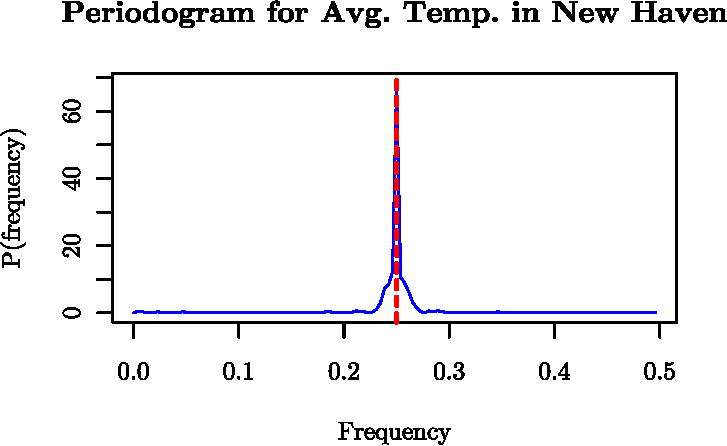
\includegraphics{Homework2_files/figure-latex/unnamed-chunk-4-1} \end{center}

The periodogram has its dominant peak at frequency \(f = 0.250\), so
\[
s = \mathrm{round}\!\left(\frac{1}{0.250}\right) = 4.
\]
Therefore, the New Haven average temperature series is modeled with quarterly seasonality (\(s = 4\)).

\newpage

\subsection{Problem 2 (b)}\label{problem-2-b}

\begin{problem}[Problem 2 (b)]
Report the three fitted models.
\end{problem}

\begin{Shaded}
\begin{Highlighting}[]
\CommentTok{\# Build regressors and fit the three models.}
\NormalTok{t    }\OtherTok{\textless{}{-}} \FunctionTok{time}\NormalTok{(Y)}
\NormalTok{t2   }\OtherTok{\textless{}{-}}\NormalTok{ t}\SpecialCharTok{\^{}}\DecValTok{2} \SpecialCharTok{/} \FunctionTok{factorial}\NormalTok{(}\DecValTok{2}\NormalTok{)}
\NormalTok{cs1  }\OtherTok{\textless{}{-}} \FunctionTok{cos}\NormalTok{(}\DecValTok{2} \SpecialCharTok{*}\NormalTok{ pi }\SpecialCharTok{*}\NormalTok{ t }\SpecialCharTok{/}\NormalTok{ s)}
\NormalTok{sn1  }\OtherTok{\textless{}{-}} \FunctionTok{sin}\NormalTok{(}\DecValTok{2} \SpecialCharTok{*}\NormalTok{ pi }\SpecialCharTok{*}\NormalTok{ t }\SpecialCharTok{/}\NormalTok{ s)}
\NormalTok{cs2  }\OtherTok{\textless{}{-}} \FunctionTok{cos}\NormalTok{(}\DecValTok{4} \SpecialCharTok{*}\NormalTok{ pi }\SpecialCharTok{*}\NormalTok{ t }\SpecialCharTok{/}\NormalTok{ s)}
\NormalTok{sn2  }\OtherTok{\textless{}{-}} \FunctionTok{sin}\NormalTok{(}\DecValTok{4} \SpecialCharTok{*}\NormalTok{ pi }\SpecialCharTok{*}\NormalTok{ t }\SpecialCharTok{/}\NormalTok{ s)}
\NormalTok{fit1 }\OtherTok{\textless{}{-}} \FunctionTok{lm}\NormalTok{(Y }\SpecialCharTok{\textasciitilde{}}\NormalTok{ t }\SpecialCharTok{+}\NormalTok{ cs1 }\SpecialCharTok{+}\NormalTok{ sn1)}
\NormalTok{fit2 }\OtherTok{\textless{}{-}} \FunctionTok{lm}\NormalTok{(Y }\SpecialCharTok{\textasciitilde{}}\NormalTok{ t }\SpecialCharTok{+}\NormalTok{ t2 }\SpecialCharTok{+}\NormalTok{ cs1 }\SpecialCharTok{+}\NormalTok{ sn1)}
\NormalTok{fit3 }\OtherTok{\textless{}{-}} \FunctionTok{lm}\NormalTok{(Y }\SpecialCharTok{\textasciitilde{}}\NormalTok{ t }\SpecialCharTok{+}\NormalTok{ t2 }\SpecialCharTok{+}\NormalTok{ cs1 }\SpecialCharTok{+}\NormalTok{ sn1 }\SpecialCharTok{+}\NormalTok{ cs2 }\SpecialCharTok{+}\NormalTok{ sn2)}

\CommentTok{\# See model summaries.}
\FunctionTok{summary}\NormalTok{(fit1)}
\end{Highlighting}
\end{Shaded}

\begin{verbatim}
## 
## Call:
## lm(formula = Y ~ t + cs1 + sn1)
## 
## Residuals:
##     Min      1Q  Median      3Q     Max 
## -17.262  -7.521  -0.115   4.648  14.960 
## 
## Coefficients:
##              Estimate Std. Error t value Pr(>|t|)
## (Intercept)  4.232756  56.200355   0.075    0.940
## t            0.003537   0.028349   0.125    0.901
## cs1         -0.044970   0.750657  -0.060    0.952
## sn1         -0.095639   0.753658  -0.127    0.899
## 
## Residual standard error: 8.572 on 256 degrees of freedom
## Multiple R-squared:  0.000136,   Adjusted R-squared:  -0.01158 
## F-statistic: 0.01161 on 3 and 256 DF,  p-value: 0.9983
\end{verbatim}

\begin{Shaded}
\begin{Highlighting}[]
\FunctionTok{summary}\NormalTok{(fit2)}
\end{Highlighting}
\end{Shaded}

\begin{verbatim}
## 
## Call:
## lm(formula = Y ~ t + t2 + cs1 + sn1)
## 
## Residuals:
##      Min       1Q   Median       3Q      Max 
## -17.2258  -7.0674   0.2296   4.2398  14.1111 
## 
## Coefficients:
##                Estimate  Std. Error t value Pr(>|t|)
## (Intercept) 5952.733985 6643.803267   0.896    0.371
## t             -5.998389    6.703292  -0.895    0.372
## t2             0.003028    0.003381   0.895    0.371
## cs1           -0.019103    0.751504  -0.025    0.980
## sn1           -0.078355    0.754197  -0.104    0.917
## 
## Residual standard error: 8.576 on 255 degrees of freedom
## Multiple R-squared:  0.00327,    Adjusted R-squared:  -0.01237 
## F-statistic: 0.2091 on 4 and 255 DF,  p-value: 0.9332
\end{verbatim}

\begin{Shaded}
\begin{Highlighting}[]
\FunctionTok{summary}\NormalTok{(fit3)}
\end{Highlighting}
\end{Shaded}

\begin{verbatim}
## 
## Call:
## lm(formula = Y ~ t + t2 + cs1 + sn1 + cs2 + sn2)
## 
## Residuals:
##      Min       1Q   Median       3Q      Max 
## -17.2611  -7.1015   0.2688   4.2093  13.9779 
## 
## Coefficients:
##                Estimate  Std. Error t value Pr(>|t|)
## (Intercept) 5914.416992 6672.746965   0.886    0.376
## t             -5.959728    6.732495  -0.885    0.377
## t2             0.003008    0.003396   0.886    0.377
## cs1           -0.017235    0.754501  -0.023    0.982
## sn1           -0.076877    0.757175  -0.102    0.919
## cs2            0.034329    0.755150   0.045    0.964
## sn2            0.137476    0.755529   0.182    0.856
## 
## Residual standard error: 8.609 on 253 degrees of freedom
## Multiple R-squared:  0.003408,   Adjusted R-squared:  -0.02023 
## F-statistic: 0.1442 on 6 and 253 DF,  p-value: 0.99
\end{verbatim}

The fitted models are:
\begin{align*}
\widehat{\textbf{Model I:}}\quad
\widehat{\text{AvgTemp}}_t
&= 4.233 + 0.004\,t - 0.045\,\cos\!\left(\frac{2\pi t}{4}\right) - 0.096\,\sin\!\left(\frac{2\pi t}{4}\right),\\[6pt]
\widehat{\textbf{Model II:}}\quad
\widehat{\text{AvgTemp}}_t
&= 5952.734 - 5.998\,t + 0.003\,\frac{t^2}{2!} - 0.019\,\cos\!\left(\frac{2\pi t}{4}\right) - 0.078\,\sin\!\left(\frac{2\pi t}{4}\right),\\[6pt]
\widehat{\textbf{Model III:}}\quad
\widehat{\text{AvgTemp}}_t
&= 5914.417 - 5.960\,t + 0.003\,\frac{t^2}{2!} - 0.017\,\cos\!\left(\frac{2\pi t}{4}\right) - 0.077\,\sin\!\left(\frac{2\pi t}{4}\right)\\
&\quad + 0.034\,\cos\!\left(\frac{4\pi t}{4}\right) + 0.137\,\sin\!\left(\frac{4\pi t}{4}\right),
\end{align*}
where \(\text{AvgTemp}_t\) denotes the New Haven average temperature at time \(t\).

\newpage

\subsection{Problem 2 (c)}\label{problem-2-c}

\begin{problem}[Problem 2 (c)]
Prepare a summary table with number of regression parameters, \(R_a^2\), AIC, AICC and BIC. Which model best explains temperature changes and why?
\end{problem}

\begin{Shaded}
\begin{Highlighting}[]
\CommentTok{\# Collect model{-}fit criteria.}
\NormalTok{fit\_table }\OtherTok{\textless{}{-}} \ControlFlowTok{function}\NormalTok{(fit) \{}
\NormalTok{  n   }\OtherTok{\textless{}{-}} \FunctionTok{length}\NormalTok{(}\FunctionTok{resid}\NormalTok{(fit))}
\NormalTok{  r   }\OtherTok{\textless{}{-}} \FunctionTok{length}\NormalTok{(}\FunctionTok{coef}\NormalTok{(fit))}
\NormalTok{  sse }\OtherTok{\textless{}{-}} \FunctionTok{sum}\NormalTok{(}\FunctionTok{resid}\NormalTok{(fit)}\SpecialCharTok{\^{}}\DecValTok{2}\NormalTok{)}
  \FunctionTok{data.frame}\NormalTok{(}
    \AttributeTok{Parameters =}\NormalTok{ r,}
    \AttributeTok{R2a  =} \FunctionTok{summary}\NormalTok{(fit)}\SpecialCharTok{$}\NormalTok{adj.r.squared,}
    \AttributeTok{AIC  =} \FunctionTok{AIC}\NormalTok{(fit) }\SpecialCharTok{/}\NormalTok{ n,}
    \AttributeTok{AICC =} \FunctionTok{log}\NormalTok{(sse }\SpecialCharTok{/}\NormalTok{ n) }\SpecialCharTok{+}\NormalTok{ ((n }\SpecialCharTok{+}\NormalTok{ r) }\SpecialCharTok{/}\NormalTok{ (n }\SpecialCharTok{{-}}\NormalTok{ r }\SpecialCharTok{{-}} \DecValTok{2}\NormalTok{)),}
    \AttributeTok{BIC  =} \FunctionTok{AIC}\NormalTok{(fit, }\AttributeTok{k =} \FunctionTok{log}\NormalTok{(n)) }\SpecialCharTok{/}\NormalTok{ n}
\NormalTok{  )}
\NormalTok{\}}
\NormalTok{comp }\OtherTok{\textless{}{-}}\NormalTok{ dplyr}\SpecialCharTok{::}\FunctionTok{bind\_rows}\NormalTok{(}
  \StringTok{\textquotesingle{}Model I\textquotesingle{}}   \OtherTok{=} \FunctionTok{fit\_table}\NormalTok{(fit1),}
  \StringTok{\textquotesingle{}Model II\textquotesingle{}}  \OtherTok{=} \FunctionTok{fit\_table}\NormalTok{(fit2),}
  \StringTok{\textquotesingle{}Model III\textquotesingle{}} \OtherTok{=} \FunctionTok{fit\_table}\NormalTok{(fit3),}
  \AttributeTok{.id =} \StringTok{\textquotesingle{}Model\textquotesingle{}}
\NormalTok{)}
\NormalTok{comp}\SpecialCharTok{$}\NormalTok{Parameters }\OtherTok{\textless{}{-}} \FunctionTok{as.integer}\NormalTok{(comp}\SpecialCharTok{$}\NormalTok{Parameters)}
\NormalTok{comp }\OtherTok{\textless{}{-}}\NormalTok{ comp }\SpecialCharTok{\%\textgreater{}\%}
\NormalTok{  dplyr}\SpecialCharTok{::}\FunctionTok{mutate}\NormalTok{(}
    \AttributeTok{R2a  =} \FunctionTok{round}\NormalTok{(R2a, }\DecValTok{3}\NormalTok{),}
    \AttributeTok{AIC  =} \FunctionTok{round}\NormalTok{(AIC, }\DecValTok{3}\NormalTok{),}
    \AttributeTok{AICC =} \FunctionTok{round}\NormalTok{(AICC, }\DecValTok{3}\NormalTok{),}
    \AttributeTok{BIC  =} \FunctionTok{round}\NormalTok{(BIC, }\DecValTok{3}\NormalTok{)}
\NormalTok{  )}
\FunctionTok{table\_latex}\NormalTok{(comp, }\AttributeTok{col\_names =} \FunctionTok{c}\NormalTok{(}\StringTok{\textquotesingle{}Model\textquotesingle{}}\NormalTok{, }\StringTok{\textquotesingle{}}\SpecialCharTok{\textbackslash{}\textbackslash{}}\StringTok{\# Parameters\textquotesingle{}}\NormalTok{, }\StringTok{\textquotesingle{}$R\_a\^{}2$\textquotesingle{}}\NormalTok{, }\StringTok{\textquotesingle{}AIC\textquotesingle{}}\NormalTok{, }\StringTok{\textquotesingle{}AICC\textquotesingle{}}\NormalTok{, }\StringTok{\textquotesingle{}BIC\textquotesingle{}}\NormalTok{))}
\end{Highlighting}
\end{Shaded}

\begin{table}[H]
\centering
\begin{tabular}{cccccc}
\toprule
Model & \# Parameters & $R_a^2$ & AIC & AICC & BIC\\
\midrule
Model I & 4 & -0.012 & 7.158 & 5.321 & 7.226\\
Model II & 5 & -0.012 & 7.162 & 5.326 & 7.245\\
Model III & 7 & -0.020 & 7.178 & 5.342 & 7.287\\
\bottomrule
\end{tabular}
\end{table}

From the comparison table:

\bgroup 
  \begin{itemize}[
    itemsep=3pt,
    parsep=0pt,
    topsep=6pt
  ]

\item All three adjusted \(R^2\) values are near zero (slightly negative), so none of these deterministic trend/seasonality models explains much variation in this New Haven quarterly-average series (we can see all of the regular \(R^2\) values are near zero as well, so that's reasonable, I think). Model I has the largest \(R_a^2\) (least negative) among the three.
\item Model I also has the smallest AIC, AICC, and BIC.

  \end{itemize}
\egroup

Therefore, \textbf{Model I} is selected: adding the quadratic and higher-harmonic terms does not improve fit enough to offset the complexity penalty, although, again, it's not like Model I is great either.

\end{document}
